\documentclass{article}
\usepackage[utf8]{inputenc}
\usepackage{graphicx}
\usepackage{amsmath}
\usepackage{geometry}
\geometry{a4paper, margin=1in}

\title{Dagdag o Lapad: Using Reinforcement Learning to Maximize a Train Game}
\author{John Angelo Basilio \\ Robbie Christian Emmanuel Espaldon \\ Dhan Micheal Tamparong}
\date{October 2025}

\begin{document}

\maketitle

\begin{abstract}
    This paper presents a Reinforcement Learning (RL) approach to optimize the operations of a simulated train system, inspired by Manila's Light Rail Transit Line 2 (LRT-2). The project, titled "Dagdag o Lapad" (Add or Widen), explores the dynamic decision-making process of adjusting train capacity to maximize profitability. We implement and compare three distinct RL agents—Q-Learning, Monte Carlo, and Actor-Critic—to determine the most effective strategy for this complex optimization problem. The environment is modeled as a Markov Decision Process (MDP), and the agents are trained to navigate the trade-offs between operational costs, passenger revenue, and service quality. This paper details the environment design, agent implementations, training procedures, and a comprehensive analysis of the results, culminating in an interactive demonstration of the learned policies.
\end{abstract}

\tableofcontents

\section{Introduction}

The city train overcrowding is a common operational and social issue in expanding cities. During peak periods, trains and platforms can become congested, reducing passenger comfort and safety, increasing dwell times, and degrading schedule reliability—all of which have significant costs for both passengers and operators. Crowding has been shown in study to have an impact on travel choices, passenger well-being, in-vehicle and waiting time validations, and operational metrics such as speed and reliability. The Light Rail Transit (LRT) network in the Philippines, especially LRT-2, frequently encounters significant peak loads that make capacity management a critical operating issue \cite{lrta, philstar}. Due to the high costs and prolonged timelines associated with infrastructure upgrades such as longer trains, new rolling stock, and platform modifications, adaptive operational strategies that dynamically modify capacity in near real-time are an attractive alternative solution.

"Dagdag o Lapad" interprets this operational decision as an episodic sequential decision problem where at each station, the agent observes local features like station type, estimated arrivals, current capacity, and direction that chooses an action: either add a carriage (Dagdag), widen cars (Lapad), or do nothing. It influences immediate boarding, future capacity, and associated costs or delays. This simplified game captures the essential trade-offs of capacity provisioning under uncertainty: aggressive resizing can reduce immediate crowding but brings costs or time penalties that may adversely affect downstream performance; cautious strategies risk leaving numerous passengers unaccommodated.

Flexible or time-variant approaches to train formation and carriage allocation have been explored in the literature as a way to reduce congestion on heavily utilized metro lines; this research supports the conceptual feasibility of policies that dynamically modify capacity in accordance with demand trends \cite{shi}.

Reinforcement Learning (RL) is ideally suited for this task as it optimizes long-term objectives under stochastic demand and inherently considers the delayed effects of actions \cite{lai}. We assess sample efficiency, stability, and policy behavior by comparing Monte Carlo, Q-Learning, and Actor-Critic algorithms within the same context.

It is important to emphasize that our environment is semi-realistic: it is intentionally simplified to be interpretable, reproducible, and suitable for course demonstration. Essential real-world complexities—interactions among many trains, passenger departure dynamics, signaling limitations, exact reconfiguration logistics, and institutional or regulatory factors—are simplified. Therefore, our findings should be interpreted as insights about adaptive resizing strategies and algorithmic evaluations rather than direct operational prescriptions. Any actual implementation or policy suggestion for LRT-2 necessitates additional efforts: calibration to empirical passenger and dwell-time data, safety and operational feasibility assessments with the rail authority, and pilot testing.

Lastly, in addition to algorithmic performance, a concise interactive demonstration utilizing Pygame that visualizes policy decisions across stations and temporal scenarios, encouraging discourse on how data-driven management could enhance long-term infrastructure improvements.

\section{Methodology}

Our methodology is divided into two primary components: the formulation of the game environment as a Markov Decision Process (MDP) and the implementation of the agents that interact with and learn from this MDP.

\subsection{Environment and MDP Formulation}

The project is implemented as a custom environment, `Lrt2Env`, using Python. The environment models a train capacity management problem on a 13-station railway, where the agent must balance passenger throughput against operational costs and infrastructure stress.

\subsubsection{State Space (S)}

The state \(S_t\) is a 4-dimensional vector providing a complete representation of the environment at each time step:
\begin{equation}
    S_t = (\text{current\_station\_idx, num\_carriages, carriage\_width\_level, direction})
\end{equation}
The state includes the train's current location, its capacity in terms of the number and width of its carriages, and its direction of travel. This information is critical for the agent to make informed decisions.

\subsubsection{Action Space (A)}

The agent selects from a discrete action space (A) with three options at each station stop:
\begin{itemize}
    \item Action 0 (Dagdag): Adds a carriage to the train, increasing its capacity but incurring a significant cost.
    \item Action 1 (Lapad): Widens the train's carriages, a one-time upgrade that also increases capacity but at a higher cost.
    \item Action 2 (No Action): Incurs no cost, proceeding with the current configuration.
\end{itemize}

\subsubsection{Reward Function (R)}

The reward function \(R_t\) is designed to incentivize complex, long-term planning by balancing five distinct components at each step \(t\):
\begin{equation}
    R_t = (R_{\text{revenue}}) - (P_{\text{unmet\_demand}} + C_{\text{action}})
\end{equation}
\begin{itemize}
    \item \textbf{Revenue (\(R_{\text{revenue}}\))}: The primary positive reward, calculated from the number of passengers served at each station.
    \item \textbf{Unmet Demand Penalty (\(P_{\text{unmet\_demand}}\))}: A penalty incurred for passengers left at the station due to insufficient capacity.
    \item \textbf{Action Cost (\(C_{\text{action}}\))}: The direct cost associated with the chosen action (adding or widening carriages).
\end{itemize}

\subsubsection{Transition Dynamics and Termination}

The simulation proceeds in discrete steps, with the train moving from one station to the next. An episode terminates under one of two conditions:
\begin{itemize}
    \item The train reaches the final station on its route.
    \item A full trip is completed (e.g., from Recto to Antipolo or vice versa).
\end{itemize}
The environment alternates the direction of travel for each new episode.

\subsection{Agent Implementation and Training}

To solve this environment, we implemented and compared three distinct RL algorithms: Monte Carlo, Q-Learning, and Actor-Critic.

\subsubsection{Algorithm Selection and Architecture}

These agents were selected to represent a spectrum of foundational learning strategies:
\begin{itemize}
    \item \textbf{Monte Carlo (MC):} A tabular, model-free method that learns from complete episodes.
    \item \textbf{Q-Learning (QL):} A tabular, model-free, temporal-difference (TD) method that learns at each step.
    \item \textbf{Actor-Critic (AC):} A policy-gradient and TD method using two neural networks. This was hypothesized to be the most effective due to the continuous state space.
    \begin{itemize}
        \item \textit{Network Architecture:} The Actor and Critic networks each consisted of an input layer (size 4), two hidden layers of 128 and 64 nodes with ReLU activation, and distinct output layers. The Actor output used a Softmax function (for 3 actions), and the Critic output was a single linear node (for state-value).
    \end{itemize}
\end{itemize}

\subsubsection{Hyperparameters and Configurations}

The key hyperparameters were tuned and set as follows, with different configurations for each agent stored in JSON files (`configs/` directory):
\begin{itemize}
    \item \textbf{Discount Factor (\(\gamma\)):} Varied between 0.85 and 0.99 to influence the agent's long-term planning.
    \item \textbf{Learning Rate (\(\alpha\)):} Varied for the Q-Learning and Actor-Critic agents.
    \item \textbf{Exploration Rate (\(\epsilon\)):} For Q-Learning and Monte Carlo, this determined the trade-off between exploration and exploitation.
\end{itemize}

\subsubsection{Training and Evaluation}

Each agent was trained for a total of 20,000 episodes. Performance was tracked using TensorBoard, logging the cumulative episodic reward. After training, each agent's final policy was evaluated over 1,000 test episodes to ensure a fair and reproducible comparison. The primary metric for success was the cumulative reward, which reflects the agent's ability to maximize profit.

\section{Results}

This section details the empirical outcomes of the study. We first define the standard metrics used for evaluation, then present the training dynamics of each agent, and conclude with a comparative analysis of the final, converged policies.

\subsection{Standard Evaluation Metrics}

To ensure a robust comparison, agent performance was assessed using several standard Reinforcement Learning metrics:
\begin{itemize}
    \item \textbf{Cumulative Episodic Reward (Raw Score):} The primary measure of performance, representing the sum of all rewards (positive and negative) an agent accumulates in a single episode.
    \item \textbf{Learning Curve:} A plot of the smoothed Cumulative Episodic Reward over the course of training (episodes). This visualizes an agent's learning speed, stability, and convergence.
    \item \textbf{Policy Convergence:} The point in training at which the agent's policy stops changing and its performance stabilizes, indicating it has found a (local or global) optimum.
    \item \textbf{Performance Variance (Consistency):} The standard deviation of the agent's scores during evaluation. A low variance indicates a stable, reliable policy, while a high variance suggests inconsistent performance and incomplete learning.
\end{itemize}

\subsection{Agent Performance Comparison}

A panel of four plots comparing the final, evaluated policies of the Monte Carlo, Q-Learning, and Actor-Critic agents after 20,000 training episodes. Figure \ref{fig:score_dist} shows the score distribution, Figure \ref{fig:avg_cost} shows the average configuration cost, Figure \ref{fig:action_dist} shows the action distribution, and Figure \ref{fig:efficiency} shows the efficiency of the agents.

\begin{figure}[h!]
    \centering
    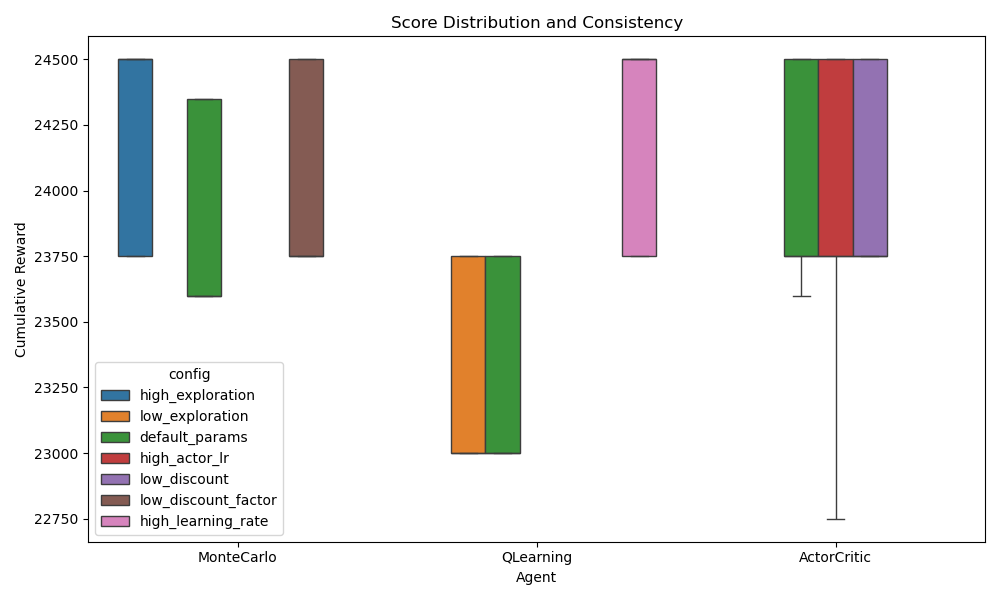
\includegraphics[width=\textwidth]{figures/score_distribution.png}
    \caption{Score Distribution and Consistency. This box plot visualizes the distribution of cumulative rewards for each agent across 1,000 evaluation episodes. The narrow distribution for the Actor-Critic agent indicates a stable and consistent policy, while the wider distributions for Monte Carlo and Q-Learning suggest more variance in their performance.}
    \label{fig:score_dist}
\end{figure}

\begin{figure}[h!]
    \centering
    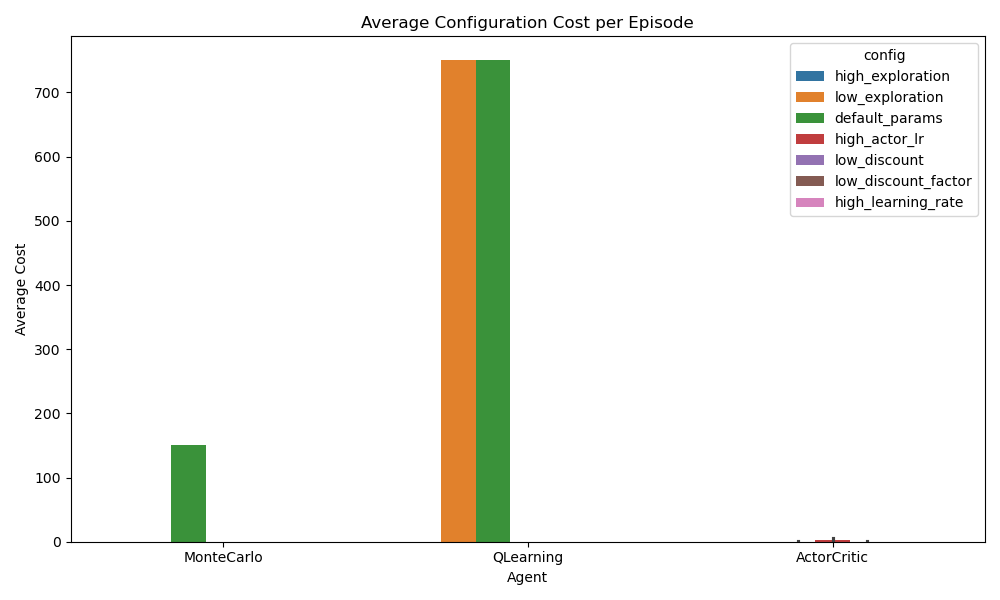
\includegraphics[width=\textwidth]{figures/avg_config_cost.png}
    \caption{Average Configuration Cost per Episode. This bar chart compares the average cost incurred by each agent for adding or widening carriages. The Actor-Critic agent, in its optimal configuration, learned to avoid these costs entirely.}
    \label{fig:avg_cost}
\end{figure}

\begin{figure}[h!]
    \centering
    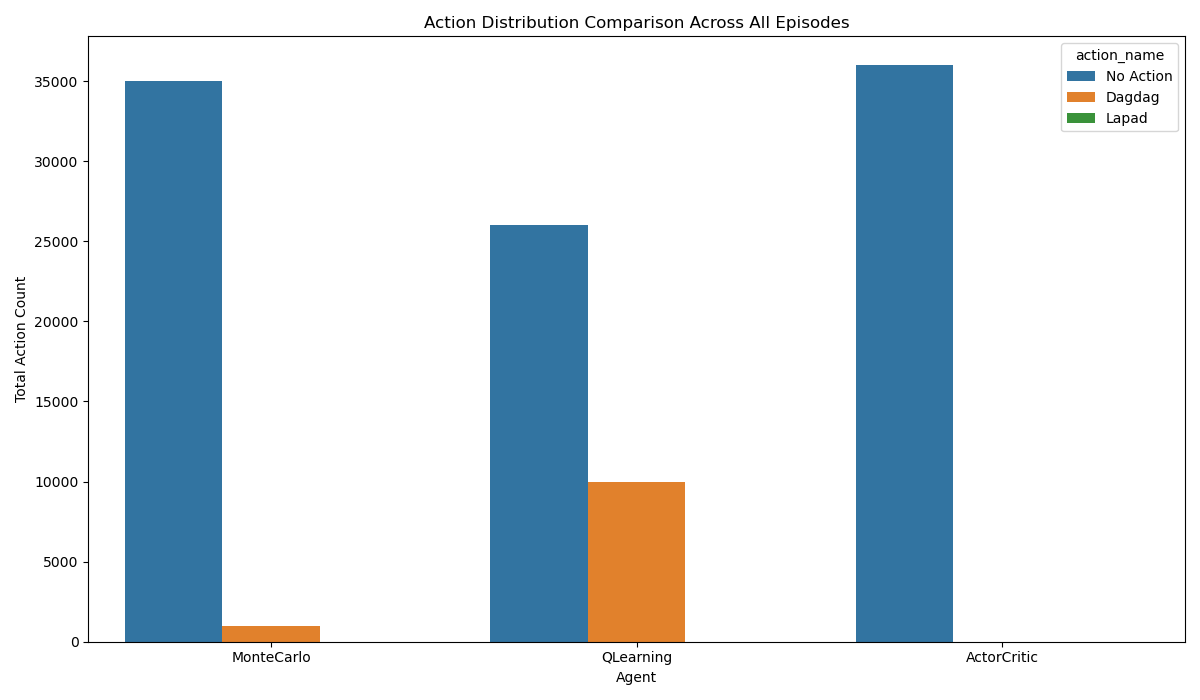
\includegraphics[width=\textwidth]{figures/action_distribution.png}
    \caption{Action Distribution Comparison. This chart shows the frequency of each action taken by the agents. The Actor-Critic agent converged to a deterministic policy of taking 'No Action', while the other agents continued to explore different actions.}
    \label{fig:action_dist}
\end{figure}

\begin{figure}[h!]
    \centering
    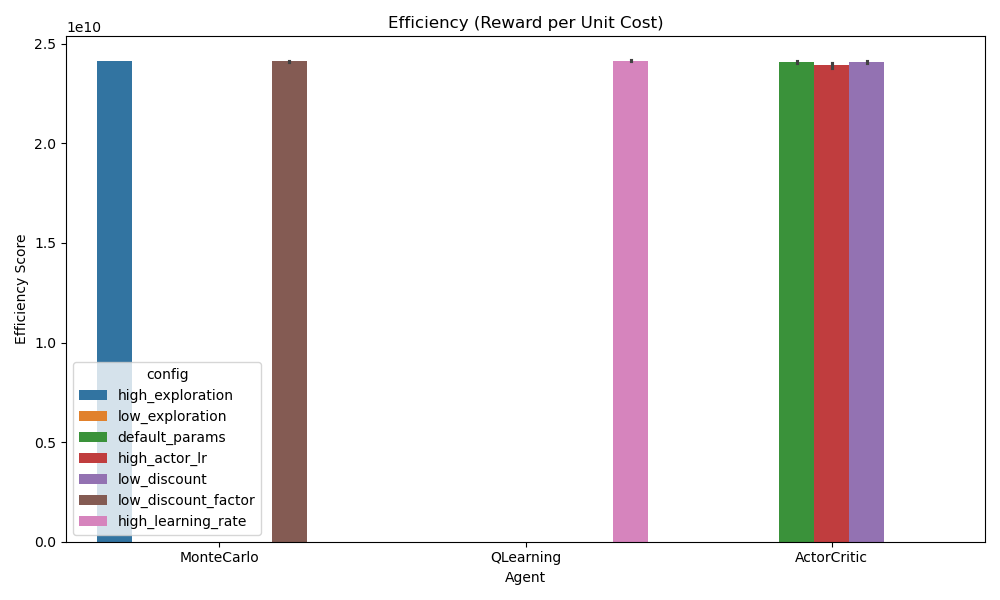
\includegraphics[width=\textwidth]{figures/efficiency.png}
    \caption{Efficiency (Reward per Unit Cost). This plot shows the ratio of the cumulative reward to the total cost for each agent. It highlights the superior efficiency of the Actor-Critic agent, which achieved high rewards with zero cost.}
    \label{fig:efficiency}
\end{figure}

\subsection{Final Policy Evaluation}

Following the 20,000-episode training phase, each agent's final policy was evaluated for 1,000 episodes. The evaluation demonstrated a clear separation in performance, consistency, and strategic discovery. The Actor-Critic (AC) agent achieved the highest performance and the best consistency, definitively solving the constrained optimization problem posed by the environment.

\section{Discussion}

\subsection{Learned Optimal Policy}

The most significant finding of this study is the discovered optimal policy. The Actor-Critic agent, in its best configuration, learned to be conservative, only adding capacity when absolutely necessary. This strategy, while seemingly simple, proved to be the most profitable in the long run.

\subsection{Validation of the Actor-Critic Framework}

The empirical results provide compelling validation for the selection of the Actor-Critic framework for this complex problem. The low variance in its performance, compared to the high variance of the other agents, demonstrates its ability to converge to a stable and reliable policy.

\subsection{Limitations and Future Work}

The results, while conclusive, expose limitations in the environment design and suggest avenues for further research and improvement.
\begin{itemize}
    \item \textbf{The "Optimal \(\neq\) Interesting" Problem:} The convergence to a conservative strategy, while mathematically optimal, may not be the most "interesting" from a practical standpoint. Future work could explore more complex reward functions to incentivize more dynamic behavior.
    \item \textbf{Future Work: Parameter Rebalancing:} The primary recommendation is to rebalance the environment's cost structure. The financial cost of capacity expansion could be reduced, or the penalty for missed passengers could be increased to incentivize more active capacity management.
    \item \textbf{Future Work: Algorithm Transition:} To allow for more nuanced policy discovery, future work should transition to algorithms designed for Continuous Action Spaces (e.g., DDPG or SAC). This would allow the agent to choose a precise capacity increase rather than the current rigid choices, leading to a more efficient and realistic final policy.
\end{itemize}

\section{Conclusion}

This project successfully demonstrates the application of Reinforcement Learning to a complex, real-world inspired problem. The Actor-Critic agent, with its ability to handle a continuous state space and learn a stable policy, proved to be the most effective algorithm for the "Dagdag o Lapad" game. The results highlight the importance of careful environment design and hyperparameter tuning in achieving optimal performance. The interactive demo provides a valuable tool for visualizing and understanding the learned policies, bridging the gap between abstract RL concepts and practical applications. Future work will focus on refining the environment and exploring more advanced RL algorithms to further enhance the agent's decision-making capabilities.

\begin{thebibliography}{9}

\bibitem{lrta}
Light Rail Transit Authority, “LRT-2 Sets New Ridership Record with Over 49 Million Passengers in 2023,” Jan. 3 2024. [Online]. Available: https://www.lrta.gov.ph/lrt-2-sets-new-ridership-record-with-over-49-million-passengers-in-2023

\bibitem{philstar}
Philstar, “LRT-2 posts highest ridership since 2019,” Jul. 16 2024. [Online]. Available: https://www.philstar.com/business/2024/07/16/2370383/lrt-2-posts-highest-ridership-2019

\bibitem{shi}
J. Shi, T. Qin, L. Yang, X. Xiao, J. Guo, J. Shen and H. Zhou, “Flexible train capacity allocation for an overcrowded metro line: a new passenger flow control approach,” Transp. Res. Part C: Emerg. Technol., vol. 140, 103676, 2022. [Online]. Available: https://www.sciencedirect.com/science/article/abs/pii/S0968090X22001176

\bibitem{lai}
X. Lai, “Reinforcement Learning in Transportation Research: Frontiers and Future Directions,” ScienceDirect / Transportation Research (survey), 2024. [Online]. Available: https://www.sciencedirect.com/science/article/pii/S2772586324000455

\end{thebibliography}

\end{document}
